\documentclass[11pt,a4paper, dvipdfmx]{article}

% margin
\usepackage[left=20mm,right=20mm,top=20mm,bottom=28.5mm,footskip=10mm,headsep=19pt]{geometry}

% packages
\usepackage{graphicx}
\usepackage{hyperref}
\usepackage{algorithmic}
\usepackage{booktabs}
\newcommand{\theHalgorithm}{\arabic{algorithm}}

% tcolorbox
\usepackage{tcolorbox}
\tcbuselibrary{breakable, skins, theorems}
\newtcbtheorem{theorem}{定理}{enhanced,frame empty,interior empty,colframe=cyan!50!white, top=8mm,
coltitle=black,fonttitle=\bfseries,colbacktitle=cyan!15!white,
borderline={0.5mm}{0mm}{cyan!50!white,dashed},
attach boxed title to top left={yshift=-4mm},
boxed title style={sharp corners=east,boxrule=1pt}}{thm}
\newtcbtheorem{definition}{定義}{enhanced,frame empty,interior empty,colframe=orange!50!white, top=8mm,
coltitle=black,fonttitle=\bfseries,colbacktitle=orange!15!white,
borderline={0.5mm}{0mm}{orange!50!white,dashed},
attach boxed title to top left={yshift=-4mm},
boxed title style={sharp corners=east,boxrule=1pt}}{def}
\newtcbtheorem{lemma}{補題}{enhanced,frame empty,interior empty,colframe=teal!50!white, top=8mm,
coltitle=black,fonttitle=\bfseries,colbacktitle=teal!15!white,
borderline={0.5mm}{0mm}{teal!50!white,dashed},
attach boxed title to top left={yshift=-4mm},
boxed title style={sharp corners=east,boxrule=1pt}}{lem}
\newtcbtheorem{assumption}{仮定}{enhanced,frame empty,interior empty,colframe=magenta!50!white, top=8mm,
coltitle=black,fonttitle=\bfseries,colbacktitle=magenta!15!white,
borderline={0.5mm}{0mm}{magenta!50!white,dashed},
attach boxed title to top left={yshift=-4mm},
boxed title style={sharp corners=east,boxrule=1pt}}{assump}
\tcolorboxenvironment{proof}{
  fonttitle=\bfseries,
  enhanced,
  top=0mm,
  boxrule=0pt,frame empty,
  borderline west={4pt}{0pt}{cyan!20!white},
  coltitle=blue,
  colback=white,
  sharp corners
}

% math macros
\usepackage{mymacros}

\title{テンプレート}
\author{masayoshi64}
\date{\today}

\begin{document}

\maketitle

\section{マクロ}
\[\R, \1, \Abb, \cA\]
\[\xhat, \xbar, \xtld\]
\[\argmin, \argmax\]
\[\veps, \vGam\]
\[\Expec[\mu]{X}, \Prob[\mu]{X \geq 0}, \Var[\mu]{X}\]
\[\pmx{
        a & b                \\
        c & d
    }\]
\[\dist, \proj, \conv, \iid, \vspan, \sign, \range \]
\[\psd{n}, \pd{n}\]
\[\kl{a}{b}, \opnorm{A}, \frobnorm{A}, \infnorm{B}, \set{a, b, c}, \floor{a}, \ceil{a}\]

\section{定理環境}
\begin{definition}{感動の定義}{def1}
    感動の定式化
\end{definition}
定理~\ref{thm:theorem1}を示す.
\begin{assumption}{感動の仮定}{assump1}
    感動の条件
\end{assumption}
\begin{theorem}{感動の定理}{theorem1}
    感動の主張
\end{theorem}
\begin{proof}
    以下の補題を用いる.
    \begin{lemma}{それなりに感動の補題}{lemma1}
        それなりに感動の主張
    \end{lemma}
    感動の証明
\end{proof}

\section{画像}
dvipdfmxオプションを使うのを忘れずに.
\begin{figure}[htbp]
    \centering
    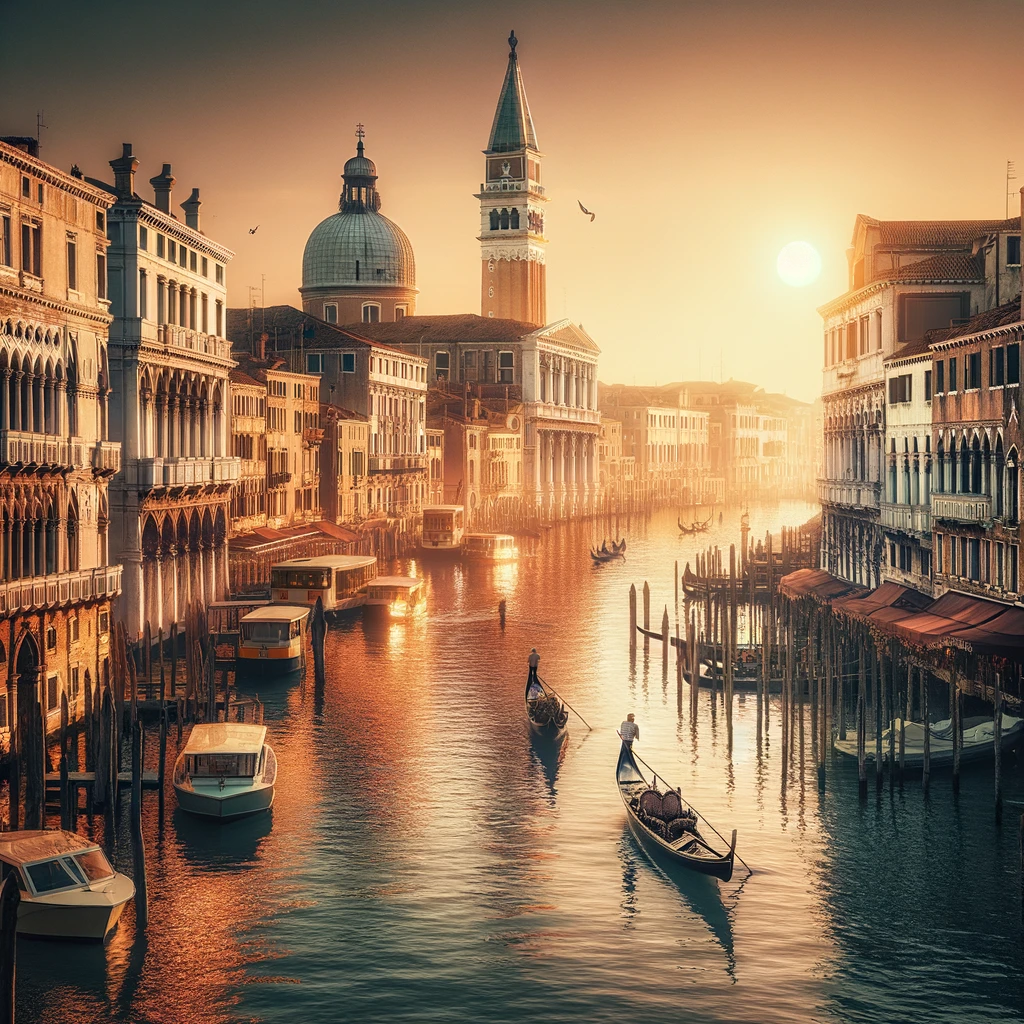
\includegraphics[width=0.5\textwidth]{figs/test.png}
    \caption{図1}
    \label{fig:fig1}
\end{figure}

\section{表}
booktabsパッケージを使う.
\begin{table}[h]
    \caption{表1}
    \label{table:table1}
    \centering
    \begin{tabular}{lcc}
        \toprule
        A  & B  & C  \\
        \midrule
        a  & b  & c  \\
        aa & bb & cc \\
        \bottomrule
    \end{tabular}
\end{table}

\section{引用}
\cite{jacot2018neural}によると...\\
...である~\cite{rafailov2023direct}.

\bibliography{main}
\bibliographystyle{plain}

\end{document}


